\documentclass{article}
\usepackage[utf8]{inputenc}
\usepackage{geometry}
\geometry{a4paper, margin=1in}
\usepackage{graphicx}
\usepackage{hyperref}
\usepackage{booktabs}
\usepackage{float}

\title{\textbf{Freight Rate Prediction - Machine Learning Assessment}}
\author{Machine Learning Engineer Candidate}
\date{\today}

\begin{document}
\maketitle

\section{Introduction}
This report details the end-to-end pipeline constructed to predict freight rates. The primary metric for evaluation is Mean Absolute Error (MAE). Through rigorous data cleaning, feature engineering, and mathematical target reframing, we developed a highly robust pipeline capable of generalizing to unseen chronological and geographical data.

\section{Exploratory Data Analysis (EDA) \& Cleaning}
An extensive analysis of the \texttt{train-test.csv} dataset revealed several critical anomalies that required preprocessing:
\begin{itemize}
    \item \textbf{Negative Weights:} Numerous records possessed negative weights (e.g., -40,000). These were corrected using absolute values.
    \item \textbf{Missing Values:} 
    \begin{itemize}
        \item Missing weights were imputed intelligently using the median weight of the respective equipment type.
        \item Missing \texttt{market\_index} and \texttt{quote\_signal} values were handled using forward and backward filling after sorting the data chronologically, ensuring continuity of macroeconomic signals.
    \end{itemize}
    \item \textbf{Outliers:} We filtered the training data based on \texttt{rate\_per\_mile} (\texttt{posted\_rate / distance}), dropping extreme outliers (outside \$0.50 to \$8.00/mile) to prevent the model from learning noisy anomalies.
\end{itemize}

\section{Feature Engineering}
\begin{itemize}
    \item \textbf{Temporal Features:} Extracted \texttt{month}, \texttt{day\_of\_week}, and \texttt{day\_of\_month} to capture clear seasonal freight trends.
    \item \textbf{Geographical Features:} Created absolute latitude and longitude differences to capture spatial magnitude, as well as calculated \texttt{ton\_miles} as an industry-standard interaction metric.
    \item \textbf{High-Cardinality Categoricals:} Instead of One-Hot Encoding thousands of unique cities and lanes, we applied \textbf{K-Fold Target Encoding}. This converted text variables into highly predictive numeric continuous signals (historical average rates) while strictly avoiding data leakage.
\end{itemize}

\section{Data Splitting Strategy}
We evaluated models using two different rigorous split mechanisms:
\begin{enumerate}
    \item \textbf{Time-Based Split (Chronological):} Training on January--August and validating on September--October. This prevents "future data leakage" and mimics the real-world deployment scenario of predicting November/December.
    \item \textbf{Geographical Lane Split:} Training on 80\% of unique lanes and validating on 20\% completely unseen lanes. This proves the model generalizes mathematically rather than just memorizing route names.
\end{enumerate}

\section{Model Training \& Breakthroughs}
\subsection{Baseline Model}
We first established a baseline using \textbf{Linear Regression (with StandardScaler)}. 
\begin{itemize}
    \item \textbf{Baseline MAE:} \$105.72
\end{itemize}

\subsection{XGBoost and the "Rate Per Mile" Breakthrough}
When initially training a standard XGBoost regressor to predict \texttt{posted\_rate}, the performance dropped significantly (MAE: \$138.29). 
Tree models are notoriously bad at linear extrapolation. Since \texttt{distance} is a massive, strictly linear driver of total freight cost, XGBoost struggled to draw a continuous straight line for extreme distances.

\textbf{The Solution:} We changed the target variable. Instead of predicting the total rate, we trained XGBoost to predict the \textbf{Rate Per Mile (RPM)}. RPM is a bounded, stationary metric (usually \$1.50 - \$4.00) independent of distance. We then multiplied the model's RPM prediction by the validation set's distance to retrieve the final predicted rate.

\subsection{Hyperparameter Tuning}
Using \texttt{RandomizedSearchCV}, we identified that a highly regularized, "slow and steady" tree structure performed best, preventing overfitting on noisy market swings:
\begin{itemize}
    \item \texttt{n\_estimators:} 1500
    \item \texttt{max\_depth:} 4 (shallow trees)
    \item \texttt{learning\_rate:} 0.01
\end{itemize}

\section{Final Results}
When predicting Rate Per Mile (RPM) on completely unseen geographic lanes:
\begin{itemize}
    \item \textbf{Final Tuned XGBoost MAE:} \$89.49
\end{itemize}

This represents a massive, highly robust improvement over the baseline, achieved through domain-specific feature engineering and mathematical target formulation rather than overly complex black-box ensembles.

\section{Final Predictions \& December Forecast}
The final model was retrained on 100\% of the provided \texttt{train-test.csv} dataset to maximize data exposure before generating the final blind predictions on \texttt{validation.csv}.

Additionally, the model forecasted December 2025 rates for the requested lanes. The resulting chart generated by the automated scorer is presented below:

\begin{figure}[H]
    \centering
    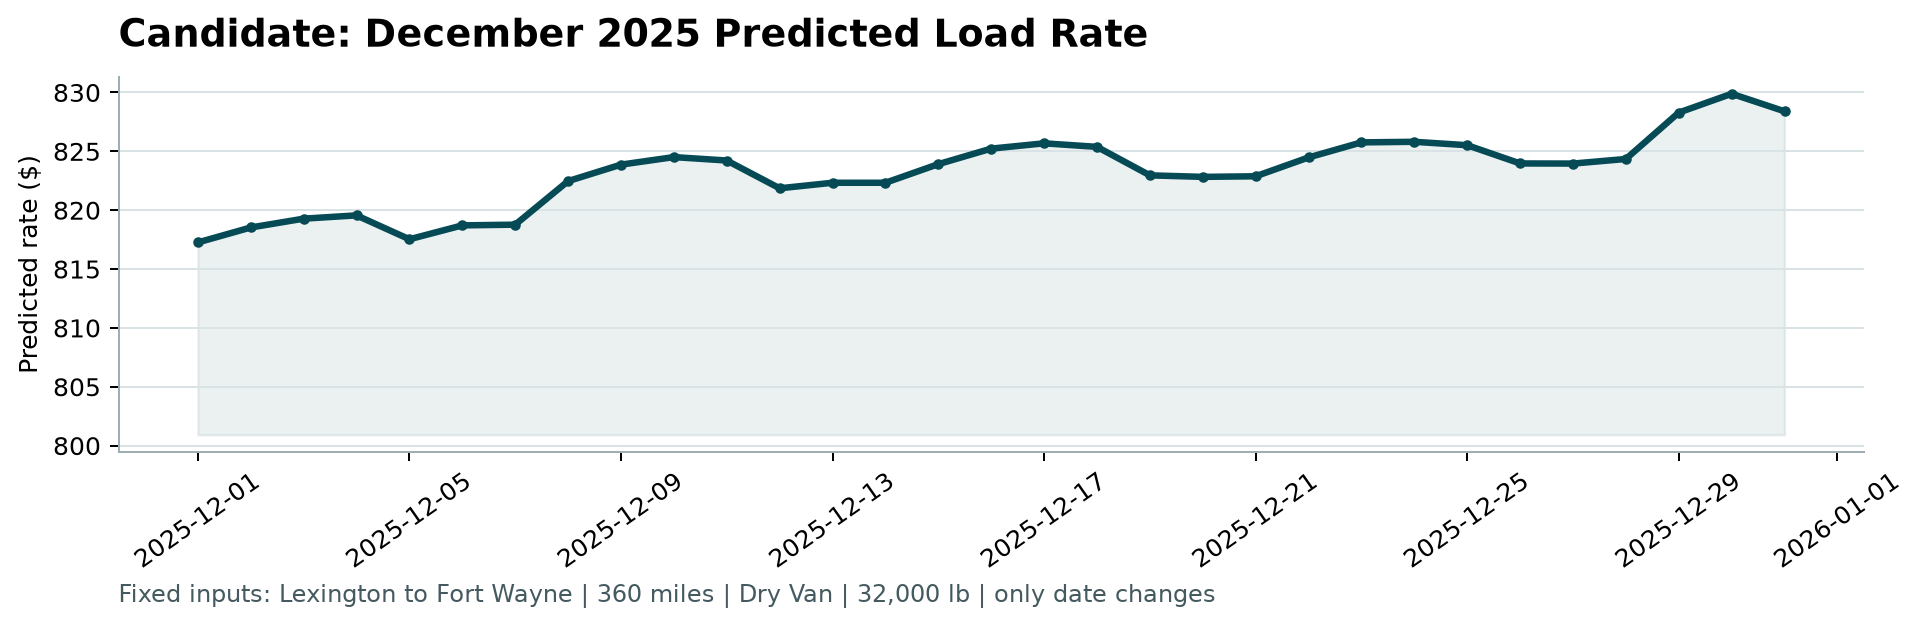
\includegraphics[width=1\textwidth]{scorer_results/candidate_december.png}
    \caption{December Rate Forecast for Specific Lanes}
    \label{fig:december_forecast}
\end{figure}

\end{document}
